\section{Methods} \label{sec:methods}

We intuitively motivate our \A heuristics and its improvements
in~\cref{sec:intuition}. Then we formally define the general chaining seed
heuristic~(\cref{sec:heuristic}) that encompases \emph{inexact matches},
\emph{chaining}, and \emph{gap costs}~(\cref{fig:heuristics}). Next, we
introduce the \emph{match pruning}~(\cref{sec:pruning}) improvement and
integrate our \A algorithm with the \emph{diagonal-transition}
optimization~(\cref{sec:dt}). We present a practical
algorithm~(\cref{sec:computation}), implementation~(\cref{sec:impl}) and
proofs of correctness~(\cref{sec:proofs}).

\begin{figure}[H]
    \centering
%    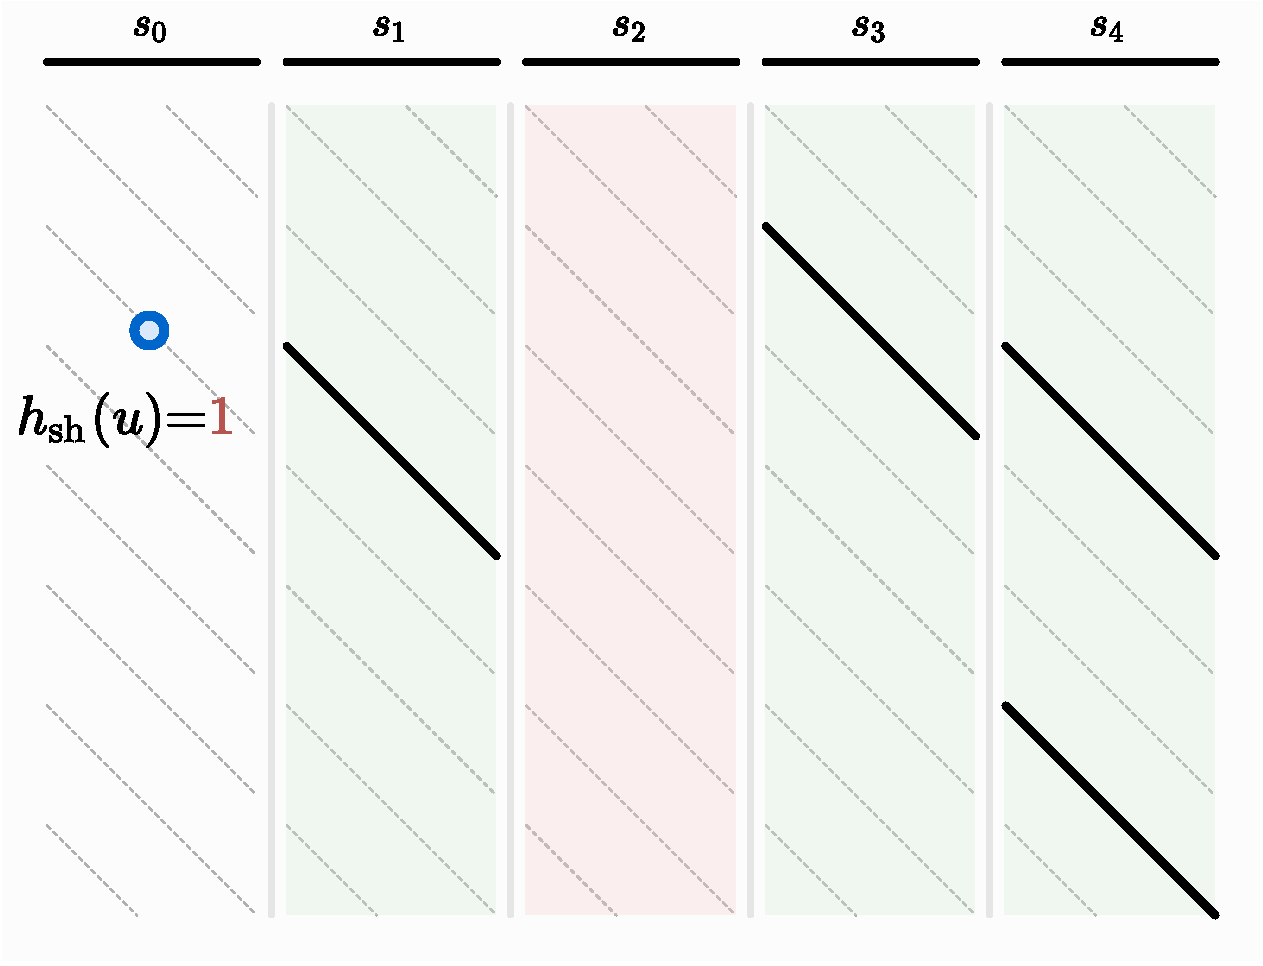
\includegraphics[width=0.24\linewidth]{imgs/heuristic-diagrams/sh.pdf}

    \subfloat[\Sh]{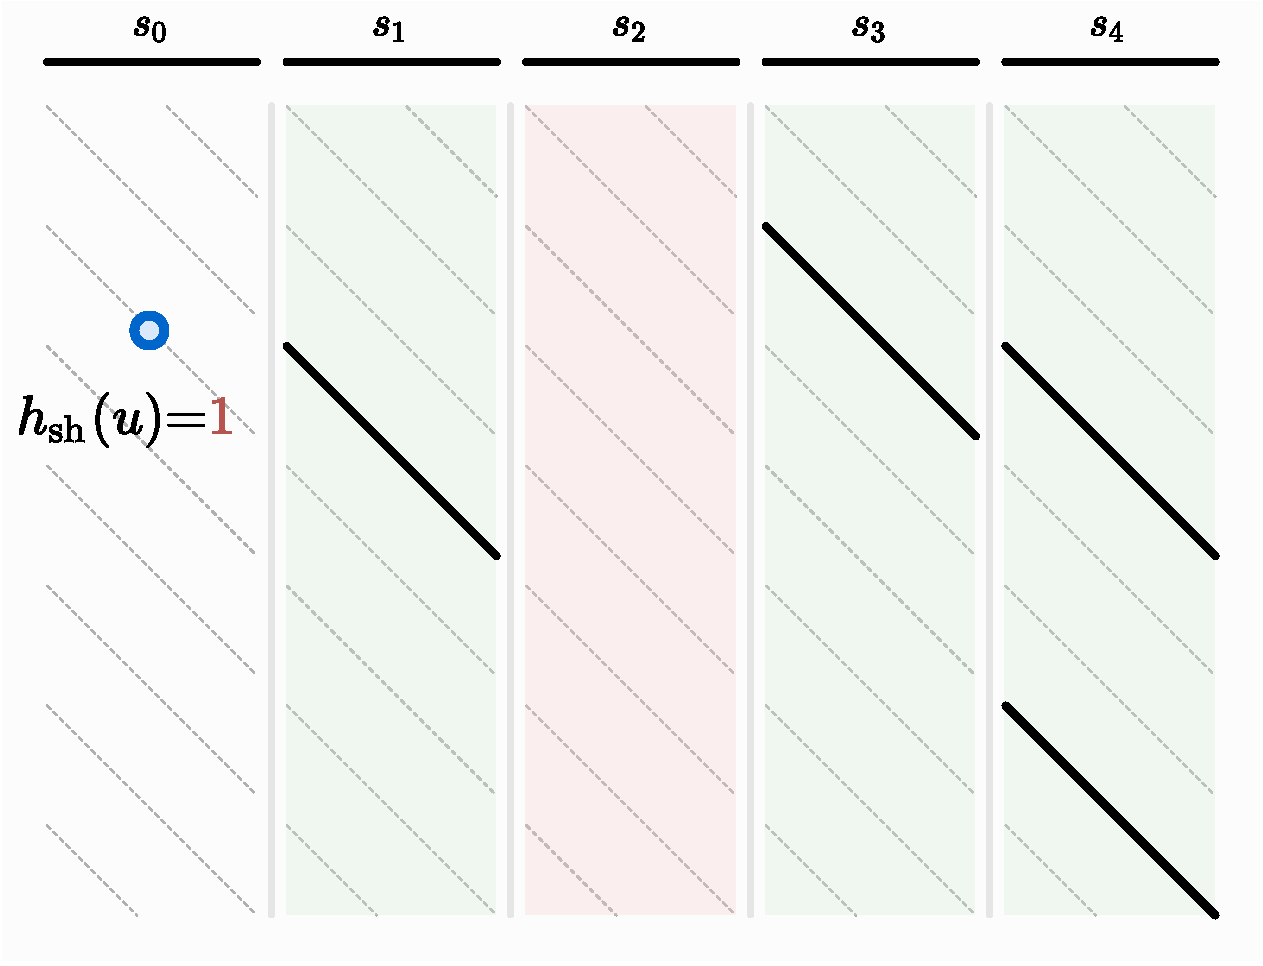
\includegraphics[width=0.4\linewidth]{imgs/heuristic-diagrams/sh.pdf}\label{fig:sh}}
    \hfill
    \subfloat[\Csh]{
\includegraphics[width=0.4\linewidth]{imgs/heuristic-diagrams/csh.pdf}\label{fig:csh}}
    \\ %\hfill
    \subfloat[\Gch]{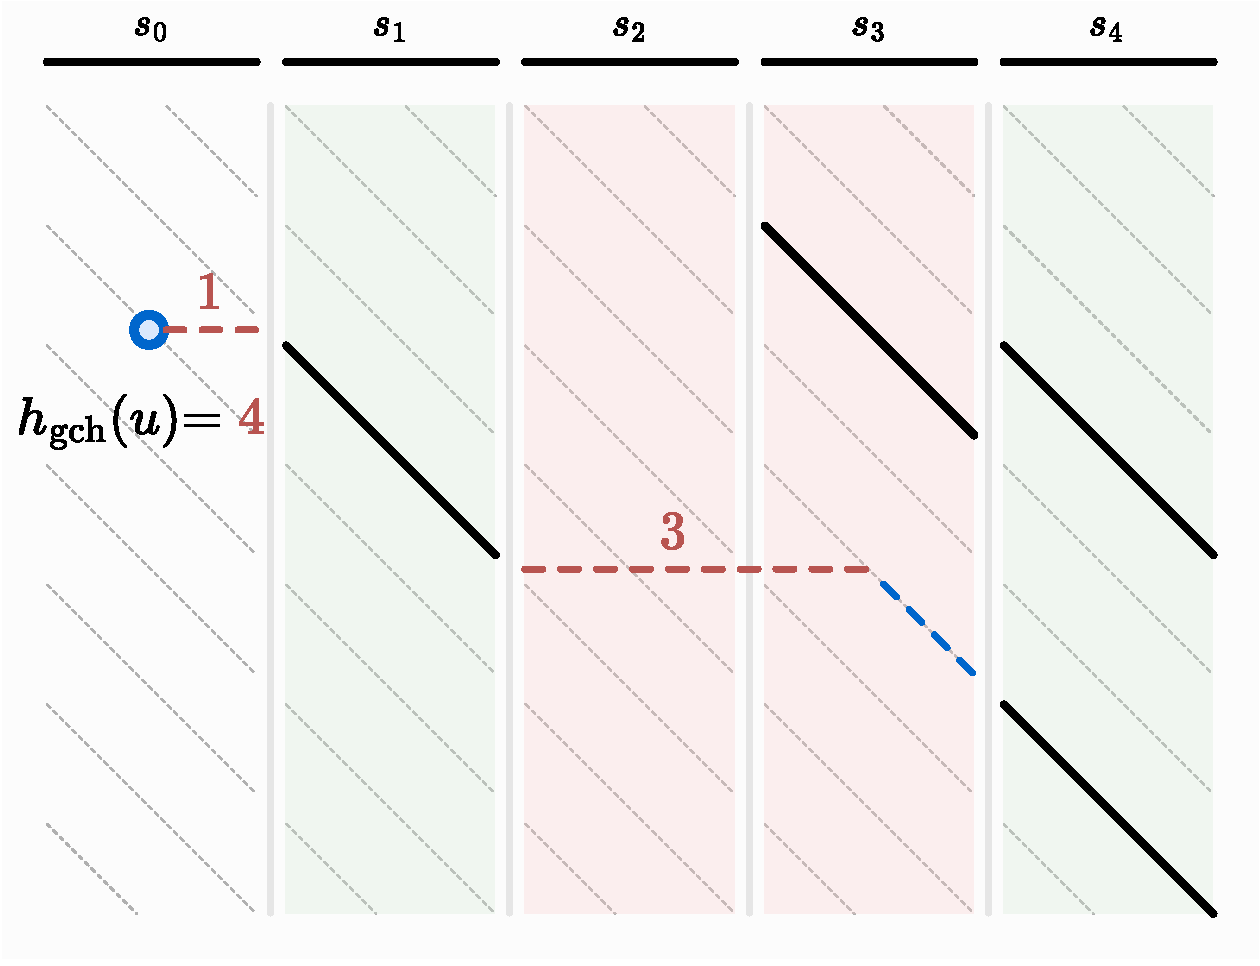
\includegraphics[width=0.4\linewidth]{imgs/heuristic-diagrams/gch.pdf}\label{fig:gch}}
    \hfill
    \subfloat[\CSH + match pruning]{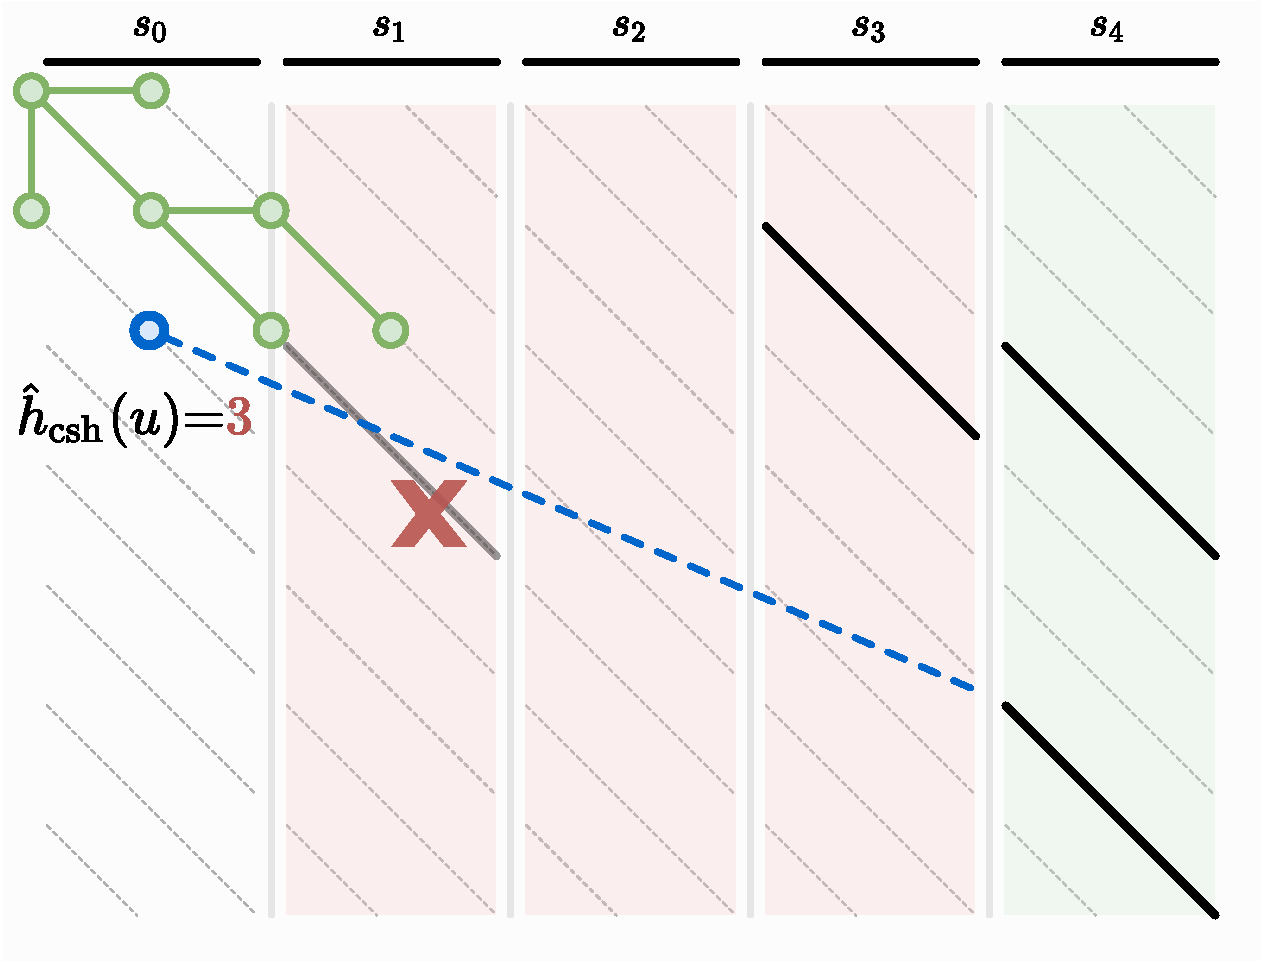
\includegraphics[width=0.4\linewidth]{imgs/heuristic-diagrams/pruning.pdf}\label{fig:pruning}}

    \caption[Family of chaining seed heuristics]{\textbf{Demonstration of \sh, \csh, \gch, and match pruning.}
      Sequence $A$ is split into $5$ seeds (horizontal black segments \seed) on
      top. Each seed is exactly matched in $B$ (diagonal black segments \match).
      The heuristic is evaluated at state $u$ (blue circles \bluecircle), based
      on the $4$ remaining seeds. The heuristic value is based on a maximal
      chain of matches (green columns \greencolumn\ for seeds with
      matches; red columns \redcolumn\ otherwise). Dashed lines denote chaining
      of matches.
      %
      \protect\subref{fig:sh} The \sh $\hsh(u) {=} 1$ is the number of remaining
      seeds that do not have matches (only $s_2$).
      %
      \protect\subref{fig:csh} The \csh $\hcsh(u) {=} 2$ is the number of
      remaining seeds without a match ($s_2$ and $s_3$) on a path going only
      down and to the right containing a maximal number of matches.
      %
      \protect\subref{fig:gch} The \gch $\hgch(u) {=} 4$ is minimal cost of a
      chain, where the cost of joining two matches is the maximum of the number
      of not matched seeds and the gap cost between them. Red dashed lines
      denote gap costs.
      %
      \protect\subref{fig:pruning} Once the start or end of a match is expanded
      (green circles \greencircle), the match is \emph{pruned} (red cross
      \cross), and future computations of the heuristic ignore it. $s_1$ is
      removed from the maximum chain of matches starting at $u$ so $\hcshS(u)$
      increases by~$1$.}
    \label{fig:heuristics}
\end{figure}

\subsection{Overview} \label{GLOBALsec:intuition}

% Shortest path task, \A
In order to find a minimal cost alignment of $A$ and $B$, we use the \A
algorithm to find a shortest path from the starting state $v_s{=}\st 00$ to the
target state $v_t{=}\st nm$ in the alignment graph. We present two heuristic functions,
the \sh and the \csh, and prove that they are admissible, so that \A always finds a
shortest path.

% SH
To define the \sh $\hsh$\,, we split $A$ into short, non-overlapping substrings
(\emph{seeds}) of fixed length $k$. Since the whole of sequence $A$ has to be
aligned, each of the seeds also has to be aligned somewhere. If
a seed cannot be \emph{exactly} matched in $B$ without mistakes, then at least
one edit has to be made to align it. We first compute all positions in
$B$ where each seed from $A$ matches exactly. Then, a
lower bound on the edit distance between the remaining suffixes $A_{\geq i}$ and
$B_{\geq j}$ is given by the number of seeds entirely contained in $A_{\geq i}$
that do not match anywhere in $B$. An example is shown in \cref{GLOBALfig:sh}.

% CSH
We improve the \sh by enforcing that the seed matches occur in the same order as
their seeds occur in $A$, \ie, they form a \emph{chain}. Now, the number of upcoming
errors is at least the minimal number of remaining seeds that cannot be aligned
on a single path to the target. The \csh $\hcsh$ equals the number of remaining
seeds minus the maximum length of a chain of matches, see \cref{GLOBALfig:csh}.

% inexact matches
To scale to larger error rates, we generalize both heuristics to use
\emph{inexact matches}. For each seed from $A$, our algorithm finds all its
inexact matches in $B$ with cost at most $1$. Then, not using any match of a
seed will require at least $r{=}2$ edits for the seed to be eventually aligned.

% pruning
Finally, we use \emph{match pruning}: once we find a shortest path to a state
$v$, no shorter path to that state is possible. Since we are only looking for a
single shortest path, we may ignore any other path going to $v$. In particular,
when we are evaluating the heuristic $h$ in some state $u$ preceding $v$, and
$v$ is at the start of a match, all paths containing the match are excluded, and
thus we may simply ignore (\emph{prune}) this match for future computations of
the heuristic. This increases the value of the heuristic, as shown in \cref{GLOBALfig:pruning}, and leads to a
significant reduction of the number of states being expanded by the \A.

\subsection{\Sh and \csh}\label{GLOBALsec:seedh}

We start with the formal definitions of seeds and matches that are the basis of
our heuristic functions and algorithms.

\paragraph{Seeds} We split the sequence $A$ into a set of consecutive
non-overlapping substrings~(\emph{seeds}) $\seeds=\{s_0, s_1, s_2, \dots
s_{\lfloor n/k \rfloor-1}\}$, such that each seed $s_l = \substr A{lk}{lk{+}k}$
has length $k$. After aligning the first $i$ letters of $A$, the information for
the heuristic will come from the \emph{remaining} seeds ${\seeds_{\geq i} :=
\{s_l \in \seeds \mid lk \geq i\}}$ contained in the suffix $A_{\geq i}$.

\paragraph{Seed alignment} An \emph{alignment} of a seed $s = \substr A{i}{i+k}$
is a path $\pi_s$ in the alignment graph $G$ from a state $u{=}\st ij$ to a state
$v{=}\st{i{+}k}{j'}$, where $i$ is the start and $i{+}k$ is the end of $s$. We refer
to the cost of the alignment $\pi_s$ as $\cost(\pi_s)$.

\paragraph{Matches}
In order to only consider good alignments of seeds, we fix a threshold cost $r$
called the \emph{seed potential}. We define a \emph{match} $m$ as an alignment of
a seed with cost ${\cost(m) < r}$. For each seed $s$, the set of all of its
matches is $\matches_s$. The inequality is strict so that $\matches_s=\emptyset$
implies that aligning the seed will incur cost at least $r$. Let $\matches =
\bigcup_s \matches_s$ denote the set of all matches. With $\spot{=}1$ we allow only
\emph{exact} matches, while for $\spot{=}2$ we allow both exact and
\emph{inexact} matches with one edit. In this paper we do not consider larger
$\spot$.

Next, we define two heuristic functions: 

\begin{definition}[\Sh]
  Given a set of matches $\matches$ with costs less than $r$, the \emph{\sh} $\hshM$\, in
  a state $u{=}\st ij$ is the minimal total cost to independently align all remaining
  seeds: each seed is either matched or incurs cost $r$ if it cannot be matched in
  $\matches$:
  \begin{equation}
    \hshM(u) := \sum_{s\in \seeds_{\geq i}} \begin{cases}
    \min_{m\in \matches_s} \cost(m) &\text{if $\matches_s \neq \emptyset$}, \\
    r &\text{otherwise.}
    \end{cases}
    \label{GLOBALeq:sh}
  \end{equation}
\end{definition}

\begin{definition}[\Csh]
  Given a set of matches $\matches$ of costs less than $r$, the \emph{\csh} $\hcshM$\,
  in a state $u{=}\st ij$ is the minimal cost to jointly align each remaining
  seed on a single path in the alignment graph:
  \begin{equation}
    \hcshM(u) := \min_{\pi \in G \path u{v_t}}  \sum_{s\in \seeds_{\geq i}}
    \begin{cases}
    \cost(\pi_s) &\text{if $\pi_s \in \matches_s$}, \\
    r &\text{otherwise.}
    \end{cases}
    \label{GLOBALeq:csh}
  \end{equation}
  where $\pi$ runs over all paths from $u$ to $v_t$, and $\pi_s$ is the shortest
  part of the path $\pi$ that is an alignment of the seed $s$.
\end{definition}

We abbreviate $\hsh := \hshM$ and $\hcsh := \hcshM$ when $\matches$ is the set of all
matches of cost strictly less than $r$. For such $\matches$, both heuristics guarantee
finding an optimal alignment.

%% ADMISSIBLE
\begin{thm}\label{GLOBALthm:admissible}
  The \sh $\hsh$\, and the \csh $\hcsh$\, are \emph{admissible}.
\end{thm}
\begin{proof}
  Let $u{=}\st ij$ be any state in the alignment graph $G(V,E)$, and let $\pi$ be any
  path from $u$ to the target $t$. A heuristic $h$ is admissible if $h(u) \leq
  \cost(\pi)$ for all $u\in V$ and for all paths $\pi$.

  We first show that $\hcsh$ is admissible. Each remaining seed in $\seeds_{\geq i}$
  is aligned somewhere by the path $\pi$. Since the seeds do not overlap, their
  shortest alignments in $\pi$ do not have overlapping edges. Each edge in
  $\pi$ has a non-negative cost, and hence $\sum_{s\in \seeds_i} \cost(\pi_s) \leq \cost(\pi)$.
  The alignment $\pi_s$ of each seed either has cost less than $\spot$ and
  equals a match in $\matches_s$, or it has cost at least $\spot$ otherwise. Together
  this implies that $\hcshM$ is a lower bound on the remaining cost $\h(u)$:
  \begin{equation}
    \begin{split}
    &\hcshM(u) = \min_{\pi \in G \path ut}  \sum_{s\in \seeds_{\geq i}}
    \begin{cases}
    \cost(\pi_s) &\text{if $\pi_s \in \matches_s$}, \\
    r &\text{otherwise.}
    \end{cases}\\
    &\leq \min_{\pi \in G \path ut}  \sum_{s\in \seeds_{\geq i}} \cost(\pi_s)
    \leq \min_{\pi \in G \path ut}  \cost(\pi) = \h(u).
    \end{split}
  \end{equation}
  We now show that the \sh $\hshM(u)$ is bounded above by $\hcshM(u)$, so that
  it is also admissible:
  \begin{align*}
    \hshM(u) &= \sum_{s\in \seeds_{\geq i}}
      \begin{cases}
      \min_{m\in \matches_s}\cost(m) &\text{if $\matches_s\neq \emptyset$}, \\
      r &\text{otherwise.}
      \end{cases}\\
    &\leq  \sum_{s\in \seeds_{\geq i}} \min_{\pi \in G \path ut}
      \begin{cases}
      \cost(\pi_s) &\text{if $\pi_s \in \matches_s$}, \\
      r &\text{otherwise.}
      \end{cases}\\
    &\leq \min_{\pi \in G \path ut}  \sum_{s\in \seeds_{\geq i}}
      \begin{cases}
      \cost(\pi_s) &\text{if $\pi_s \in \matches_s$}, \\
      r &\text{otherwise.}
      \end{cases} 
    = \hcshM(u).
  \end{align*}
\end{proof}

As a consequence of the proof,
$\hcsh(u)$ dominates $\hsh(u)$, that is, ${\hcsh(u) \geq \hsh(u)}$ for all $u$.
Hence $\hcsh(u)$ usually expands fewer states, at the cost of
being more complex to compute.

\subsection{Match pruning} \label{sec:pruning}

In order to reduce the number of states expanded by the \A~algorithm, we apply
the \emph{multiple-path pruning} observation: once a shortest path to a state
has been found, no other path to this state could possibly improve the global
shortest path~\citep{poole2017artificial}. As soon as \A~expands the start or
end of a match, we \emph{prune} it, so that the heuristic in preceding states no
longer benefits from the match, and they get deprioritized by \A. We define
\emph{pruned} variants of all our heuristics that ignore pruned matches:

\begin{definition}[Pruning heuristic]
   Let $\Expanded$ be the set of expanded states during the \A~search, and let
   $\prunedmatches$ be the set of matches that were not pruned, i.e. those
   matches not starting or ending in an expanded state. We say that $\hat h :=
   h^\prunedmatches$ is a \emph{pruning heuristic} version of $h$.
\end{definition}

The hat over the heuristic function ($\hat h$) denotes the implicit dependency
on the progress of the \A, where at each step a different $h^\prunedmatches$ is
used. Our modified \A algorithm~(\cref{sec:astar-code})
works for pruning heuristics by ensuring that the $f$-value of a state is
up-to-date before expanding it, and otherwise \emph{reorders} it in the priority
queue. Even though match pruning violates the admissibility of our heuristics
for some nodes, we prove that \A is sill guaranteed to find a shortest
path~(\cref{sec:pruning-proof}). To this end, we show that our pruning
heuristics are \emph{\wah{}s}~(\cref{dfn:weak-admissible}) in the sense that
they are admissible on at least one path from $v_s$ to $v_t$.

\begin{restatable}{thm}{thmpartialadmissibledfn}\label{thm:weak-admissible-dfn}
  \A with a \wah finds a shortest path.
\end{restatable}

\begin{restatable}{thm}{thmpartialadmissibleh}\label{thm:weak-admissible-h}
  The pruning heuristics $\hshS$\,, $\hcshS$\,, $\hgchS$\, are \wa.
\end{restatable}

Pruning will allow us to scale
near-linearly with sequence length, without sacrificing optimality of the
resulting alignment.

\subsection{Computing the heuristic}\label{sec:computation}

We present an algorithm to efficiently compute our heuristics (pseudocode
in~\cref{sec:heuristic-code}). At a high level, we rephrase the minimization of
costs (over paths) to a maximization of \emph{scores} (over chains of matches).
We initialize the heuristic by precomputing all seeds, matches, potentials and a
\emph{contours} data structure used to compute the maximum number of matches on
a chain. During the \A~search, the heuristic is evaluated in all explored
states, and the contours are updated whenever a match gets pruned.

\paragraph{Scores} The \emph{score of a match} $m$ is
$\matchscore(m){:=}r{-}\matchcost(m)$ and is always positive. The \emph{score of
a $\preceq_p$-chain} $m_1\preceq_p \dots \preceq_p m_l$ is the sum of the scores
of the matches in the chain. We define the chain score of a match $m$ as
\begin{equation}
S_p(m):=\max_{m\preceq_p m_1\preceq_p\dots \preceq_p m_l\preceq_p v_t}\big\{\matchscore(m) + \dots + \matchscore(m_l)\big\}.
\label{eq:chain}
\end{equation}
Since $\preceq_p$ is a partial order, $S_p$ can be computed with
base case ${S_p(m_\omega) = 0}$ and the recursion
\begin{equation}
S_p(m) = \matchscore(m) + \max_{m\preceq_p m' \preceq v_t} S_p(m').
\label{eq:chainscore}
\end{equation}
We also define the chain score of a state $u$ as the maximum chain score over
succeeding matches $m$: $S_p(u) = \max_{u\preceq_p m \preceq_p v_t} S_p(m)$, so that
\cref{eq:chainscore} can be rewritten as $S_p(m) = \matchscore(m) +
S_p(\matchend(m))$.

\begin{figure}[t]
  \centering
  \subfloat[SH]{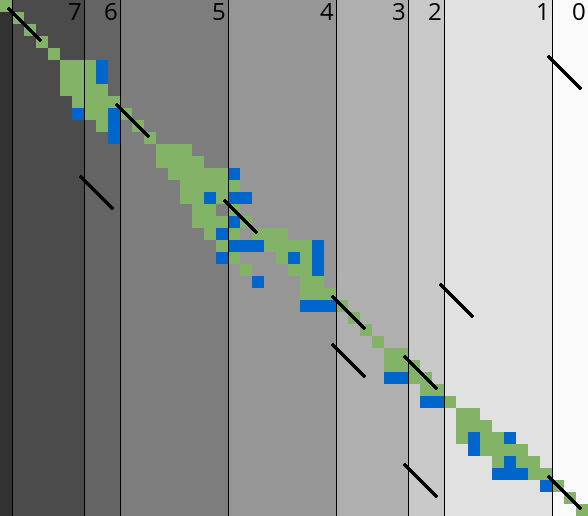
\includegraphics[width=0.32\linewidth]{imgs/layers/sh-noprune.png}\label{fig:layers-sh}}
  \hfill
  \subfloat[CSH]{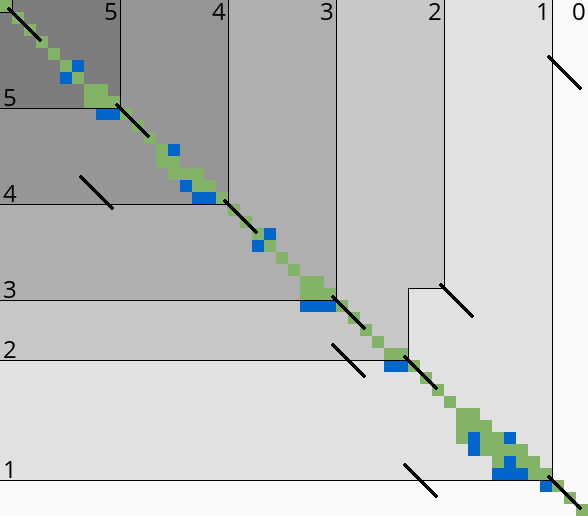
\includegraphics[width=0.32\linewidth]{imgs/layers/csh-noprune.png}\label{fig:layers-csh}}
  \hfill
  \subfloat[\GCH]{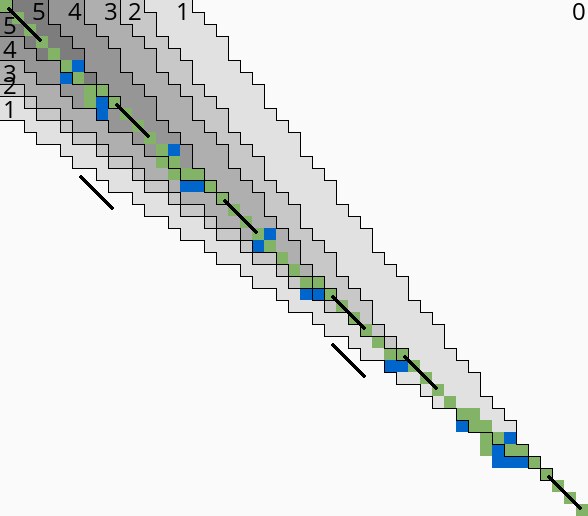
\includegraphics[width=0.32\linewidth]{imgs/layers/gcsh-noprune.png}\label{fig:layers-gcsh}}
  \\
  \subfloat[SH + pruning]{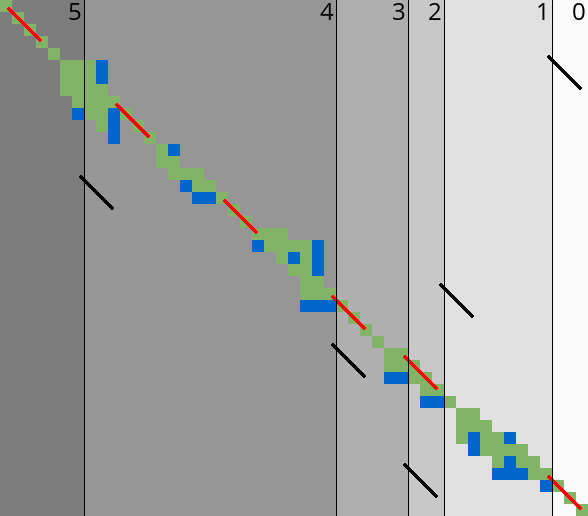
\includegraphics[width=0.32\linewidth]{imgs/layers/sh.png}\label{fig:layers-sh-pruning}}
  \hfill
  \subfloat[CSH + pruning]{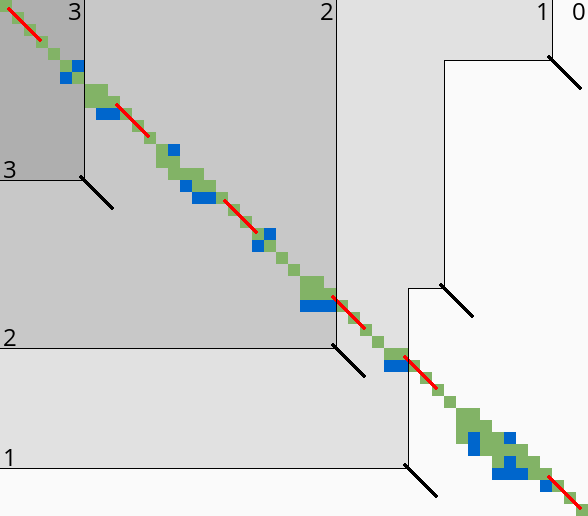
\includegraphics[width=0.32\linewidth]{imgs/layers/csh.png}\label{fig:layers-csh-pruning}}
  \hfill
  \subfloat[\GCH +
  pruning]{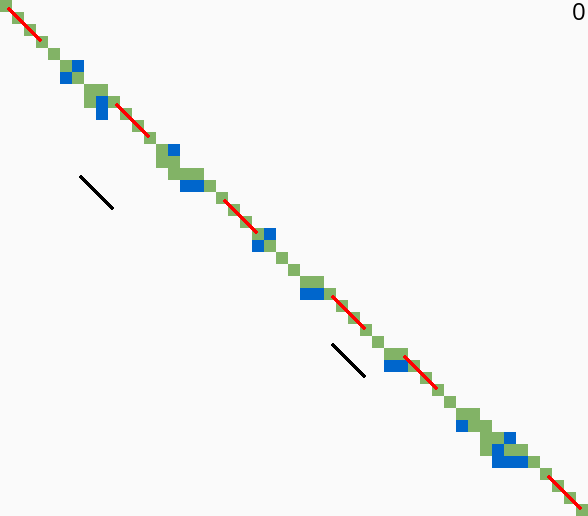
\includegraphics[width=0.32\linewidth]{imgs/layers/gcsh.png}\label{fig:layers-gcsh-pruning}}
  \caption[Contours and layers of different seed heuristics]{\textbf{Contours and layers of different heuristics after aligning}
  ($n{=}48$, $m{=}42$, $r{=}1$, $k{=}3$, edit distance $10$). Exact matches are
  black diagonal segments~(\blackmatch{}). The background colour indicates
  $S_p(u)$, the maximum number of matches on a $\preceq_p$-chain from $u$ to the
  end starting, with $S_p(u) = 0$ in white. The thin black boundaries of these
  regions are \emph{Contours}. The states of layer $\layer_\ell$ \emph{precede}
  contour $\ell$. Expanded states are green~(\greensquare{}), open states
  blue~(\bluesquare{}), and pruned matches red~(\redmatch{}). Pruning matches
  changes the contours and layers. \GCH ignores matches $m{\npreceq_T}v_t$.}
  \label{fig:contours}
\end{figure}


The following theorem allows us to rephrase the heuristic in terms of
potentials and scores for heuristics that use $\gamma {=} \seedcost$ and respect
the order of the seeds, which is the case for $\hsh$ and $\hcsh$ (proof
in~\cref{app:computation}):
\begin{restatable}{thm}{thmcomputation}\label{lem:computation}
$h^\matches_{p,\seedcost}(u) = P(u) - S_p(u)$ for any partial order~$\preceq_p$
that is a refinement of $\preceq_i$ (i.e. $u\preceq_p v$ must imply $u\preceq_i
v$).
\end{restatable}

\paragraph{Layers and contours}
We compute $\hsh$ and $\hcsh$ efficiently using \emph{contours}. Let
\emph{layer} $\layer_\ell$ be the set of states $u$ with score $S_p(u) \geq
\ell$, so that $\layer_\ell \subseteq \layer_{\ell{-}1}$. The $\ell$th
\emph{contour} is the boundary of $\layer_\ell$~(\cref{fig:contours}).
Layer~$\layer_\ell$~($\ell>0$) contains exactly those states that precede a
match $m$ with score $\ell \leq S_p(m) < \ell+r$ (\cref{lem:contour} in
\cref{app:computation}).

\paragraph{Computing $S_p(u)$}
This last observation inspires our algorithm for computing chain scores. For
each layer $\layer_\ell$, we store the set
$L[i]$~of matches having score $\ell$: ${L[\ell] = \{m\in \matches \mid S_p(m) =
\ell\}}$.
%
The score $S_p(u)$ is then the highest~$\ell$ such that
layer $L[\ell]$ contains a match $m$ reachable from $u$ ($u\preceq_p m$).
%
From~\cref{lem:contour} we know that $S_p(u) \geq \ell$ if and only if one of
the layers $L[\ell']$ for $\ell'\in [\ell, \ell+r)$ contains a match preceded
by $u$. We use this to compute $S_p(u)$ using a binary search over the layers $\ell$.
%
We initialize $L[0] {=} \{m_{\omega}\}$ ($m_{\omega}$ is a fictive match at the
target $v_t$), sort all matches in $\matches$ by~$\preceq_p$, and process them in
decreasing order (from the target to the start). After computing
$S_p(\matchend(m))$, we add~$m$ to layer $S_p(m) = \matchscore(m) +
S_p(\matchend(m))$. Matches that do not precede the target ($\matchstart(m) \not
\preceq_p m_\omega$) are ignored.

\paragraph{Pruning matches from $L$}
When pruning matches starting or ending in state~$u$ in layer $\ell_u=S_p(u)$,
we remove all matches that start at $u$ from layers $L[\ell_u{-}r{+}1]$ to
$L[\ell_u]$, and all matches starting in some~$v$ and ending in~$u$ from layers
$L[\ell_v{-}r{+}1]$ to $L[\ell_v]$.

Pruning a match may change $S_p$ in layers above~$\ell_u$, so we update them
after each prune. We iterate over increasing $\ell$ starting at
$\ell_u+1$ and recompute ${\ell':=S_p(m)\leq \ell}$ for all matches $m$ in
$L[\ell]$. If $\ell' \neq \ell$, we move $m$ from $L[\ell]$ to $L[\ell']$. We
stop iterating when either $r$ consecutive layers were left
unchanged, or when all matches in $r-1+\ell-\ell'$ consecutive layers have
shifted down by the same amount $\ell-\ell'$. In the former case, no further
scores can change, and in the latter case, $S_p$ decreases by $\ell-\ell'$
for all matches with score $\geq \ell$. We remove the emptied layers
${L[\ell'+1]}$ to $L[\ell]$ so that all higher layers shift down by
$\ell-\ell'$.

\paragraph{\SH} Due to the simple structure of the \sh, we also simplify its
computation by only storing the start of each layer and the number of matches in
each layer, as opposed to the full set of matches.

\paragraph{\GCH}
\cref{lem:computation} does not apply to \gch since it uses chaining cost
$\gamma{=}\max(\gapcost(u, v), \seedcost(u,v))$ which is different from
$\seedcost(u,v)$. It turns out that in this new setting it is never optimal to chain
two matches if the gap cost between them is higher than the seed cost.
Intuitively, it is better to miss a match than to incur additional gapcost to
include it. We capture this constraint by introducing a transformation $T$ such
that $u\preceq_T v$ holds if and only if $\seedcost(u,v) \geq \gapcost(u,v)$, as
shown in~\cref{app:gapcost-proof}. Using an additional \emph{consistency}
constraint on the set of matches we can compute $\hgchM$ via $S_T$ as before.

\begin{definition}[Consistent matches]\label{dfn:consistent} %
  A set of matches $\matches$ is \emph{consistent} when for each $m\in\matches$
  (from $\st ij$ to $\st {i'}{j'}$) with $\matchscore(m) {>} 1$, for each
  \emph{adjacent} pair of existing states $(\st i{j{\pm}1}, \st{i'}{j'})$ and
  $(\st ij, \st {i'}{j'{\pm}1})$, there is an \emph{adjacent} match with corresponding start and
  end, and score at least $\matchscore(m){-}1$.
\end{definition}
This condition means that for $r{=}2$, each exact match must be adjacent to four
(or less around the edges of the graph) inexact matches starting or ending in
the same state. Since we find all matches $m$ with $\matchcost(m){<}r$, our initial set
of matches is consistent. To preserve consistency, we do not prune matches if
that would break the consistency of $\matches$.

\begin{restatable}[Gap transformation]{definition}{transformation}\label{dfn:transformation} %
  The partial order $\preceq_T$ on states is induced by comparing both
  coordinates after the \emph{gap transformation}
% Numbered because it may be referred externally.
\begin{equation*}
  T: \quad\st{i}{j}\mapsto \tst{i - j - P\st{i}{j}}{j-i-P\st{i}{j}}
\end{equation*}
\end{restatable}

\begin{restatable}{thm}{thmgapcost}\label{lem:gapcost}%
 Given a \emph{consistent} set of matches $\matches$, the \gch can be computed
 using scores in the transformed domain:
\begin{equation*}
  \hgchM(u) =
  \begin{cases}
    \Pot(u) - S_T(u) & \text{if $u\preceq_T v_t$,} \\
    \gapcost(u, v_t) & \text{if $u\npreceq_T v_t$.}
  \end{cases}
\end{equation*}
\end{restatable}

Using the transformation of the match coordinates, we can now reduce $\gscost$
to $\seedcost$ and efficiently compute \GCH in any explored state.

